\documentclass[1p]{elsarticle_modified}
%\bibliographystyle{elsarticle-num}

%\usepackage[colorlinks]{hyperref}
%\usepackage{abbrmath_seonhwa} %\Abb, \Ascr, \Acal ,\Abf, \Afrak
\usepackage{amsfonts}
\usepackage{amssymb}
\usepackage{amsmath}
\usepackage{amsthm}
\usepackage{scalefnt}
\usepackage{amsbsy}
\usepackage{kotex}
\usepackage{caption}
\usepackage{subfig}
\usepackage{color}
\usepackage{graphicx}
\usepackage{xcolor} %% white, black, red, green, blue, cyan, magenta, yellow
\usepackage{float}
\usepackage{setspace}
\usepackage{hyperref}

\usepackage{tikz}
\usetikzlibrary{arrows}

\usepackage{multirow}
\usepackage{array} % fixed length table
\usepackage{hhline}

%%%%%%%%%%%%%%%%%%%%%
\makeatletter
\renewcommand*\env@matrix[1][\arraystretch]{%
	\edef\arraystretch{#1}%
	\hskip -\arraycolsep
	\let\@ifnextchar\new@ifnextchar
	\array{*\c@MaxMatrixCols c}}
\makeatother %https://tex.stackexchange.com/questions/14071/how-can-i-increase-the-line-spacing-in-a-matrix
%%%%%%%%%%%%%%%

\usepackage[normalem]{ulem}

\newcommand{\msout}[1]{\ifmmode\text{\sout{\ensuremath{#1}}}\else\sout{#1}\fi}
%SOURCE: \msout is \stkout macro in https://tex.stackexchange.com/questions/20609/strikeout-in-math-mode

\newcommand{\cancel}[1]{
	\ifmmode
	{\color{red}\msout{#1}}
	\else
	{\color{red}\sout{#1}}
	\fi
}

\newcommand{\add}[1]{
	{\color{blue}\uwave{#1}}
}

\newcommand{\replace}[2]{
	\ifmmode
	{\color{red}\msout{#1}}{\color{blue}\uwave{#2}}
	\else
	{\color{red}\sout{#1}}{\color{blue}\uwave{#2}}
	\fi
}

\newcommand{\Sol}{\mathcal{S}} %segment
\newcommand{\D}{D} %diagram
\newcommand{\A}{\mathcal{A}} %arc


%%%%%%%%%%%%%%%%%%%%%%%%%%%%%5 test

\def\sl{\operatorname{\textup{SL}}(2,\Cbb)}
\def\psl{\operatorname{\textup{PSL}}(2,\Cbb)}
\def\quan{\mkern 1mu \triangleright \mkern 1mu}

\theoremstyle{definition}
\newtheorem{thm}{Theorem}[section]
\newtheorem{prop}[thm]{Proposition}
\newtheorem{lem}[thm]{Lemma}
\newtheorem{ques}[thm]{Question}
\newtheorem{cor}[thm]{Corollary}
\newtheorem{defn}[thm]{Definition}
\newtheorem{exam}[thm]{Example}
\newtheorem{rmk}[thm]{Remark}
\newtheorem{alg}[thm]{Algorithm}

\newcommand{\I}{\sqrt{-1}}
\begin{document}

%\begin{frontmatter}
%
%\title{Boundary parabolic representations of knots up to 8 crossings}
%
%%% Group authors per affiliation:
%\author{Yunhi Cho} 
%\address{Department of Mathematics, University of Seoul, Seoul, Korea}
%\ead{yhcho@uos.ac.kr}
%
%
%\author{Seonhwa Kim} %\fnref{s_kim}}
%\address{Center for Geometry and Physics, Institute for Basic Science, Pohang, 37673, Korea}
%\ead{ryeona17@ibs.re.kr}
%
%\author{Hyuk Kim}
%\address{Department of Mathematical Sciences, Seoul National University, Seoul 08826, Korea}
%\ead{hyukkim@snu.ac.kr}
%
%\author{Seokbeom Yoon}
%\address{Department of Mathematical Sciences, Seoul National University, Seoul, 08826,  Korea}
%\ead{sbyoon15@snu.ac.kr}
%
%\begin{abstract}
%We find all boundary parabolic representation of knots up to 8 crossings.
%
%\end{abstract}
%\begin{keyword}
%    \MSC[2010] 57M25 
%\end{keyword}
%
%\end{frontmatter}

%\linenumbers
%\tableofcontents
%
\newcommand\colored[1]{\textcolor{white}{\rule[-0.35ex]{0.8em}{1.4ex}}\kern-0.8em\color{red} #1}%
%\newcommand\colored[1]{\textcolor{white}{ #1}\kern-2.17ex	\textcolor{white}{ #1}\kern-1.81ex	\textcolor{white}{ #1}\kern-2.15ex\color{red}#1	}

{\Large $\underline{12a_{0569}~(K12a_{0569})}$}

\setlength{\tabcolsep}{10pt}
\renewcommand{\arraystretch}{1.6}
\vspace{1cm}\begin{tabular}{m{100pt}>{\centering\arraybackslash}m{274pt}}
\multirow{5}{120pt}{
	\centering
	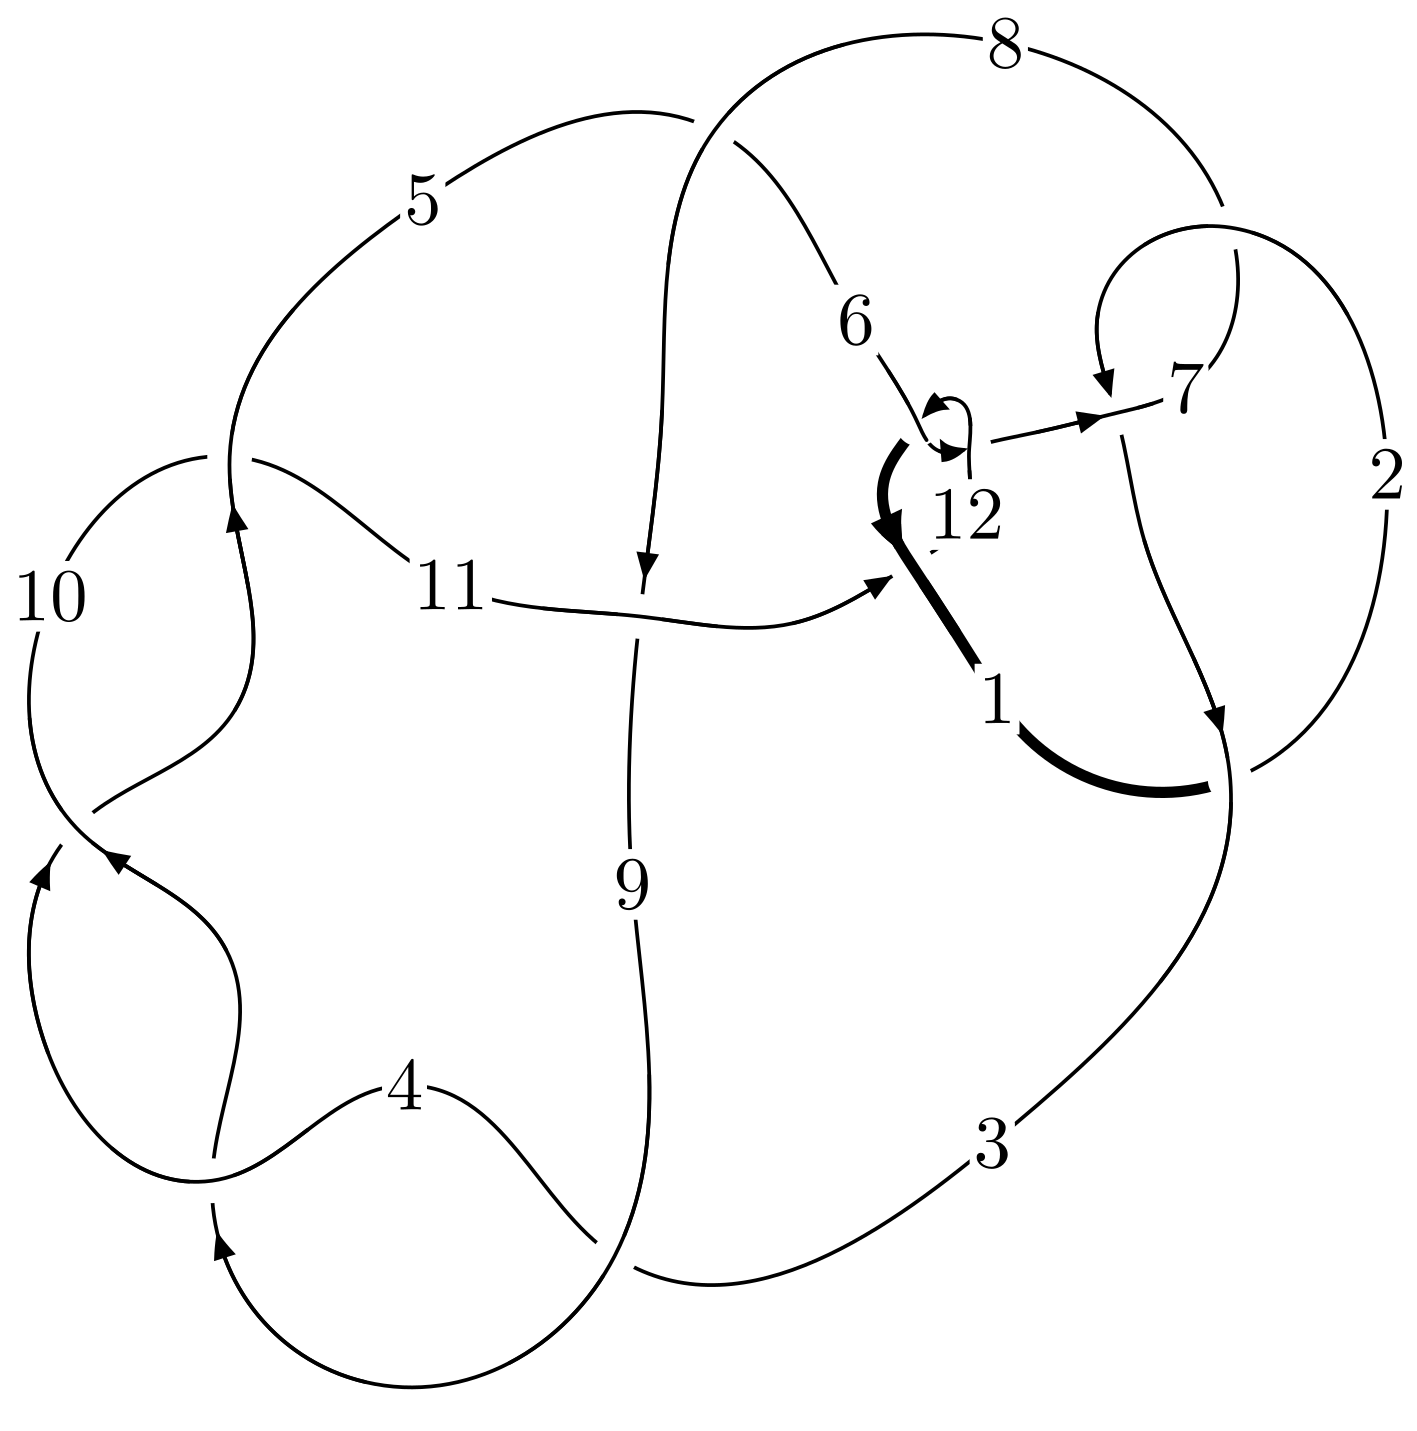
\includegraphics[width=112pt]{../../../GIT/diagram.site/Diagrams/png/1370_12a_0569.png}\\
\ \ \ A knot diagram\footnotemark}&
\allowdisplaybreaks
\textbf{Linearized knot diagam} \\
\cline{2-2}
 &
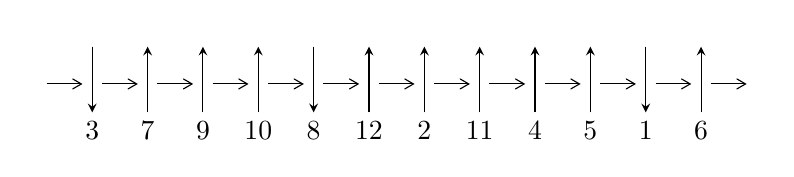
\begin{tikzpicture}[x=20pt, y=17pt]
	% nodes
	\node (C0) at (0, 0) {};
	\node (C1) at (1, 0) {};
	\node (C1U) at (1, +1) {};
	\node (C1D) at (1, -1) {3};

	\node (C2) at (2, 0) {};
	\node (C2U) at (2, +1) {};
	\node (C2D) at (2, -1) {7};

	\node (C3) at (3, 0) {};
	\node (C3U) at (3, +1) {};
	\node (C3D) at (3, -1) {9};

	\node (C4) at (4, 0) {};
	\node (C4U) at (4, +1) {};
	\node (C4D) at (4, -1) {10};

	\node (C5) at (5, 0) {};
	\node (C5U) at (5, +1) {};
	\node (C5D) at (5, -1) {8};

	\node (C6) at (6, 0) {};
	\node (C6U) at (6, +1) {};
	\node (C6D) at (6, -1) {12};

	\node (C7) at (7, 0) {};
	\node (C7U) at (7, +1) {};
	\node (C7D) at (7, -1) {2};

	\node (C8) at (8, 0) {};
	\node (C8U) at (8, +1) {};
	\node (C8D) at (8, -1) {11};

	\node (C9) at (9, 0) {};
	\node (C9U) at (9, +1) {};
	\node (C9D) at (9, -1) {4};

	\node (C10) at (10, 0) {};
	\node (C10U) at (10, +1) {};
	\node (C10D) at (10, -1) {5};

	\node (C11) at (11, 0) {};
	\node (C11U) at (11, +1) {};
	\node (C11D) at (11, -1) {1};

	\node (C12) at (12, 0) {};
	\node (C12U) at (12, +1) {};
	\node (C12D) at (12, -1) {6};
	\node (C13) at (13, 0) {};

	% arrows
	\draw[->,>={angle 60}]
	(C0) edge (C1) (C1) edge (C2) (C2) edge (C3) (C3) edge (C4) (C4) edge (C5) (C5) edge (C6) (C6) edge (C7) (C7) edge (C8) (C8) edge (C9) (C9) edge (C10) (C10) edge (C11) (C11) edge (C12) (C12) edge (C13) ;	\draw[->,>=stealth]
	(C1U) edge (C1D) (C2D) edge (C2U) (C3D) edge (C3U) (C4D) edge (C4U) (C5U) edge (C5D) (C6D) edge (C6U) (C7D) edge (C7U) (C8D) edge (C8U) (C9D) edge (C9U) (C10D) edge (C10U) (C11U) edge (C11D) (C12D) edge (C12U) ;
	\end{tikzpicture} \\
\hhline{~~} \\& 
\textbf{Solving Sequence} \\ \cline{2-2} 
 &
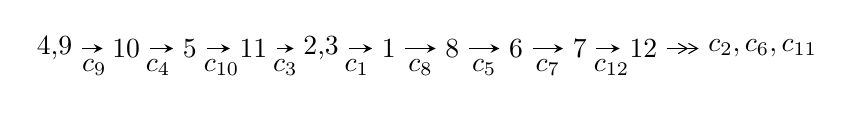
\begin{tikzpicture}[x=23pt, y=7pt]
	% node
	\node (A0) at (-1/8, 0) {4,9};
	\node (A1) at (1, 0) {10};
	\node (A2) at (2, 0) {5};
	\node (A3) at (3, 0) {11};
	\node (A4) at (65/16, 0) {2,3};
	\node (A5) at (41/8, 0) {1};
	\node (A6) at (49/8, 0) {8};
	\node (A7) at (57/8, 0) {6};
	\node (A8) at (65/8, 0) {7};
	\node (A9) at (73/8, 0) {12};
	\node (C1) at (1/2, -1) {$c_{9}$};
	\node (C2) at (3/2, -1) {$c_{4}$};
	\node (C3) at (5/2, -1) {$c_{10}$};
	\node (C4) at (7/2, -1) {$c_{3}$};
	\node (C5) at (37/8, -1) {$c_{1}$};
	\node (C6) at (45/8, -1) {$c_{8}$};
	\node (C7) at (53/8, -1) {$c_{5}$};
	\node (C8) at (61/8, -1) {$c_{7}$};
	\node (C9) at (69/8, -1) {$c_{12}$};
	\node (A10) at (11, 0) {$c_{2},c_{6},c_{11}$};

	% edge
	\draw[->,>=stealth]	
	(A0) edge (A1) (A1) edge (A2) (A2) edge (A3) (A3) edge (A4) (A4) edge (A5) (A5) edge (A6) (A6) edge (A7) (A7) edge (A8) (A8) edge (A9) ;
	\draw[->>,>={angle 60}]	
	(A9) edge (A10);
\end{tikzpicture} \\ 

\end{tabular} \\

\footnotetext{
The image of knot diagram is generated by the software ``\textbf{Draw programme}" developed by Andrew Bartholomew(\url{http://www.layer8.co.uk/maths/draw/index.htm\#Running-draw}), where we modified some parts for our purpose(\url{https://github.com/CATsTAILs/LinksPainter}).
}\phantom \\ \newline 
\centering \textbf{Ideals for irreducible components\footnotemark of $X_{\text{par}}$} 
 
\begin{align*}
I^u_{1}&=\langle 
-3 u^{33}+5 u^{32}+\cdots+b-3,\;7 u^{33}-11 u^{32}+\cdots+2 a+9,\;u^{34}-3 u^{33}+\cdots-5 u-2\rangle \\
I^u_{2}&=\langle 
-21 u^{24} a-357 u^{24}+\cdots+85 a-335,\;-2 u^{23} a-2 u^{24}+\cdots+a^2- a,\;u^{25}+u^{24}+\cdots+u-1\rangle \\
I^u_{3}&=\langle 
u^7-4 u^5+u^4+4 u^3-2 u^2+b- u,\;- u^5- u^4+3 u^3+2 u^2+a- u,\;u^8-5 u^6+7 u^4-2 u^2+1\rangle \\
\\
\end{align*}
\raggedright * 3 irreducible components of $\dim_{\mathbb{C}}=0$, with total 92 representations.\\
\footnotetext{All coefficients of polynomials are rational numbers. But the coefficients are sometimes approximated in decimal forms when there is not enough margin.}
\newpage
\renewcommand{\arraystretch}{1}
\centering \section*{I. $I^u_{1}= \langle -3 u^{33}+5 u^{32}+\cdots+b-3,\;7 u^{33}-11 u^{32}+\cdots+2 a+9,\;u^{34}-3 u^{33}+\cdots-5 u-2 \rangle$}
\flushleft \textbf{(i) Arc colorings}\\
\begin{tabular}{m{7pt} m{180pt} m{7pt} m{180pt} }
\flushright $a_{4}=$&$\begin{pmatrix}0\\u\end{pmatrix}$ \\
\flushright $a_{9}=$&$\begin{pmatrix}1\\0\end{pmatrix}$ \\
\flushright $a_{10}=$&$\begin{pmatrix}1\\- u^2\end{pmatrix}$ \\
\flushright $a_{5}=$&$\begin{pmatrix}u\\- u^3+u\end{pmatrix}$ \\
\flushright $a_{11}=$&$\begin{pmatrix}- u^2+1\\u^4-2 u^2\end{pmatrix}$ \\
\flushright $a_{2}=$&$\begin{pmatrix}-\frac{7}{2} u^{33}+\frac{11}{2} u^{32}+\cdots-\frac{29}{2} u-\frac{9}{2}\\3 u^{33}-5 u^{32}+\cdots+11 u+3\end{pmatrix}$ \\
\flushright $a_{3}=$&$\begin{pmatrix}- u\\u\end{pmatrix}$ \\
\flushright $a_{1}=$&$\begin{pmatrix}-5.50000 u^{33}+8.50000 u^{32}+\cdots-20.5000 u-6.50000\\5 u^{33}-8 u^{32}+\cdots+17 u+5\end{pmatrix}$ \\
\flushright $a_{8}=$&$\begin{pmatrix}- u^6+3 u^4-2 u^2+1\\u^8-4 u^6+4 u^4\end{pmatrix}$ \\
\flushright $a_{6}=$&$\begin{pmatrix}u^{11}-6 u^9+12 u^7-10 u^5+5 u^3\\- u^{13}+7 u^{11}-17 u^9+16 u^7-4 u^5- u^3+u\end{pmatrix}$ \\
\flushright $a_{7}=$&$\begin{pmatrix}-\frac{3}{2} u^{33}+\frac{5}{2} u^{32}+\cdots-\frac{13}{2} u-\frac{3}{2}\\2 u^{33}-3 u^{32}+\cdots+9 u+3\end{pmatrix}$ \\
\flushright $a_{12}=$&$\begin{pmatrix}\frac{7}{2} u^{33}-\frac{11}{2} u^{32}+\cdots+\frac{27}{2} u+\frac{11}{2}\\-3 u^{33}+5 u^{32}+\cdots-10 u-3\end{pmatrix}$\\&\end{tabular}
\flushleft \textbf{(ii) Obstruction class $= -1$}\\~\\
\flushleft \textbf{(iii) Cusp Shapes $= 12 u^{33}-12 u^{32}-218 u^{31}+192 u^{30}+1764 u^{29}-1284 u^{28}-8408 u^{27}+4518 u^{26}+26308 u^{25}-8142 u^{24}-56882 u^{23}+2928 u^{22}+86532 u^{21}+19602 u^{20}-91108 u^{19}-48412 u^{18}+61428 u^{17}+58604 u^{16}-19212 u^{15}-42828 u^{14}-6604 u^{13}+18558 u^{12}+10772 u^{11}-3466 u^{10}-5728 u^9-1018 u^8+1686 u^7+1004 u^6-148 u^5-386 u^4-132 u^3+52 u^2+68 u+34$}\\~\\
\newpage\renewcommand{\arraystretch}{1}
\flushleft \textbf{(iv) u-Polynomials at the component}\newline \\
\begin{tabular}{m{50pt}|m{274pt}}
Crossings & \hspace{64pt}u-Polynomials at each crossing \\
\hline $$\begin{aligned}c_{1},c_{11}\end{aligned}$$&$\begin{aligned}
&u^{34}+14 u^{33}+\cdots+2 u+1
\end{aligned}$\\
\hline $$\begin{aligned}c_{2},c_{6},c_{7}\\c_{12}\end{aligned}$$&$\begin{aligned}
&u^{34}+7 u^{32}+\cdots+2 u-1
\end{aligned}$\\
\hline $$\begin{aligned}c_{3},c_{4},c_{9}\\c_{10}\end{aligned}$$&$\begin{aligned}
&u^{34}+3 u^{33}+\cdots+5 u-2
\end{aligned}$\\
\hline $$\begin{aligned}c_{5}\end{aligned}$$&$\begin{aligned}
&u^{34}-15 u^{33}+\cdots-4575 u+358
\end{aligned}$\\
\hline $$\begin{aligned}c_{8}\end{aligned}$$&$\begin{aligned}
&u^{34}+9 u^{33}+\cdots-281 u-136
\end{aligned}$\\
\hline
\end{tabular}\\~\\
\newpage\renewcommand{\arraystretch}{1}
\flushleft \textbf{(v) Riley Polynomials at the component}\newline \\
\begin{tabular}{m{50pt}|m{274pt}}
Crossings & \hspace{64pt}Riley Polynomials at each crossing \\
\hline $$\begin{aligned}c_{1},c_{11}\end{aligned}$$&$\begin{aligned}
&y^{34}+22 y^{33}+\cdots-102 y+1
\end{aligned}$\\
\hline $$\begin{aligned}c_{2},c_{6},c_{7}\\c_{12}\end{aligned}$$&$\begin{aligned}
&y^{34}+14 y^{33}+\cdots+2 y+1
\end{aligned}$\\
\hline $$\begin{aligned}c_{3},c_{4},c_{9}\\c_{10}\end{aligned}$$&$\begin{aligned}
&y^{34}-39 y^{33}+\cdots-21 y+4
\end{aligned}$\\
\hline $$\begin{aligned}c_{5}\end{aligned}$$&$\begin{aligned}
&y^{34}+9 y^{33}+\cdots-2328229 y+128164
\end{aligned}$\\
\hline $$\begin{aligned}c_{8}\end{aligned}$$&$\begin{aligned}
&y^{34}-3 y^{33}+\cdots-79233 y+18496
\end{aligned}$\\
\hline
\end{tabular}\\~\\
\newpage\flushleft \textbf{(vi) Complex Volumes and Cusp Shapes}
$$\begin{array}{c|c|c}  
\text{Solutions to }I^u_{1}& \I (\text{vol} + \sqrt{-1}CS) & \text{Cusp shape}\\
 \hline 
\begin{aligned}
u &= \phantom{-}0.877399 + 0.216772 I \\
a &= \phantom{-}0.475747 - 0.156573 I \\
b &= \phantom{-}0.73016 + 1.40055 I\end{aligned}
 & \phantom{-}1.81473 - 6.46317 I & \phantom{-}9.54481 + 4.22755 I \\ \hline\begin{aligned}
u &= \phantom{-}0.877399 - 0.216772 I \\
a &= \phantom{-}0.475747 + 0.156573 I \\
b &= \phantom{-}0.73016 - 1.40055 I\end{aligned}
 & \phantom{-}1.81473 + 6.46317 I & \phantom{-}9.54481 - 4.22755 I \\ \hline\begin{aligned}
u &= -0.708573 + 0.517031 I \\
a &= -0.145662 + 0.387973 I \\
b &= \phantom{-}0.22304 - 2.36773 I\end{aligned}
 & -0.14844 - 13.04060 I & \phantom{-}6.35227 + 10.72030 I \\ \hline\begin{aligned}
u &= -0.708573 - 0.517031 I \\
a &= -0.145662 - 0.387973 I \\
b &= \phantom{-}0.22304 + 2.36773 I\end{aligned}
 & -0.14844 + 13.04060 I & \phantom{-}6.35227 - 10.72030 I \\ \hline\begin{aligned}
u &= \phantom{-}0.780460 + 0.363894 I \\
a &= -0.627024 - 0.012240 I \\
b &= \phantom{-}0.031716 - 1.019530 I\end{aligned}
 & \phantom{-}4.40948 + 4.16383 I & \phantom{-}12.6794 - 7.1623 I \\ \hline\begin{aligned}
u &= \phantom{-}0.780460 - 0.363894 I \\
a &= -0.627024 + 0.012240 I \\
b &= \phantom{-}0.031716 + 1.019530 I\end{aligned}
 & \phantom{-}4.40948 - 4.16383 I & \phantom{-}12.6794 + 7.1623 I \\ \hline\begin{aligned}
u &= -0.736699 + 0.432721 I \\
a &= \phantom{-}0.353503 - 0.411057 I \\
b &= -0.48051 + 1.43982 I\end{aligned}
 & \phantom{-}3.92336 - 2.16093 I & \phantom{-}12.40932 + 2.19070 I \\ \hline\begin{aligned}
u &= -0.736699 - 0.432721 I \\
a &= \phantom{-}0.353503 + 0.411057 I \\
b &= -0.48051 - 1.43982 I\end{aligned}
 & \phantom{-}3.92336 + 2.16093 I & \phantom{-}12.40932 - 2.19070 I \\ \hline\begin{aligned}
u &= -0.562396 + 0.535053 I \\
a &= -0.351346 + 0.308190 I \\
b &= -1.167160 - 0.153798 I\end{aligned}
 & -3.10387 + 1.61500 I & \phantom{-}3.93469 - 1.70541 I \\ \hline\begin{aligned}
u &= -0.562396 - 0.535053 I \\
a &= -0.351346 - 0.308190 I \\
b &= -1.167160 + 0.153798 I\end{aligned}
 & -3.10387 - 1.61500 I & \phantom{-}3.93469 + 1.70541 I\\
 \hline 
 \end{array}$$\newpage$$\begin{array}{c|c|c}  
\text{Solutions to }I^u_{1}& \I (\text{vol} + \sqrt{-1}CS) & \text{Cusp shape}\\
 \hline 
\begin{aligned}
u &= -0.369153 + 0.566173 I \\
a &= \phantom{-}0.060405 - 1.357450 I \\
b &= \phantom{-}0.522127 - 0.471400 I\end{aligned}
 & -3.66613 - 5.39835 I & \phantom{-}2.14176 + 8.12985 I \\ \hline\begin{aligned}
u &= -0.369153 - 0.566173 I \\
a &= \phantom{-}0.060405 + 1.357450 I \\
b &= \phantom{-}0.522127 + 0.471400 I\end{aligned}
 & -3.66613 + 5.39835 I & \phantom{-}2.14176 - 8.12985 I \\ \hline\begin{aligned}
u &= \phantom{-}0.478774 + 0.474535 I \\
a &= \phantom{-}0.006193 - 0.459110 I \\
b &= \phantom{-}0.318164 + 0.001013 I\end{aligned}
 & -1.82601 + 1.67416 I & \phantom{-}6.00203 - 5.31904 I \\ \hline\begin{aligned}
u &= \phantom{-}0.478774 - 0.474535 I \\
a &= \phantom{-}0.006193 + 0.459110 I \\
b &= \phantom{-}0.318164 - 0.001013 I\end{aligned}
 & -1.82601 - 1.67416 I & \phantom{-}6.00203 + 5.31904 I \\ \hline\begin{aligned}
u &= -0.184105 + 0.612147 I \\
a &= -2.40151 - 0.24206 I \\
b &= -0.085419 - 0.531958 I\end{aligned}
 & -1.68891 + 9.20421 I & \phantom{-}3.04718 - 5.89874 I \\ \hline\begin{aligned}
u &= -0.184105 - 0.612147 I \\
a &= -2.40151 + 0.24206 I \\
b &= -0.085419 + 0.531958 I\end{aligned}
 & -1.68891 - 9.20421 I & \phantom{-}3.04718 + 5.89874 I \\ \hline\begin{aligned}
u &= \phantom{-}1.43714 + 0.08661 I \\
a &= \phantom{-}0.678840 + 0.278085 I \\
b &= -0.085956 - 1.097670 I\end{aligned}
 & \phantom{-}2.03333 + 7.62639 I & \phantom{-0.000000 } 0 \\ \hline\begin{aligned}
u &= \phantom{-}1.43714 - 0.08661 I \\
a &= \phantom{-}0.678840 - 0.278085 I \\
b &= -0.085956 + 1.097670 I\end{aligned}
 & \phantom{-}2.03333 - 7.62639 I & \phantom{-0.000000 } 0 \\ \hline\begin{aligned}
u &= -0.050097 + 0.546766 I \\
a &= \phantom{-}1.46207 - 0.24634 I \\
b &= \phantom{-}0.040124 + 0.397505 I\end{aligned}
 & \phantom{-}1.94188 - 1.14446 I & \phantom{-}7.91735 + 3.10614 I \\ \hline\begin{aligned}
u &= -0.050097 - 0.546766 I \\
a &= \phantom{-}1.46207 + 0.24634 I \\
b &= \phantom{-}0.040124 - 0.397505 I\end{aligned}
 & \phantom{-}1.94188 + 1.14446 I & \phantom{-}7.91735 - 3.10614 I\\
 \hline 
 \end{array}$$\newpage$$\begin{array}{c|c|c}  
\text{Solutions to }I^u_{1}& \I (\text{vol} + \sqrt{-1}CS) & \text{Cusp shape}\\
 \hline 
\begin{aligned}
u &= -1.53119 + 0.11501 I \\
a &= \phantom{-}0.777108 + 0.261273 I \\
b &= -1.053720 - 0.389785 I\end{aligned}
 & \phantom{-}4.89311 - 3.68703 I & \phantom{-0.000000 } 0 \\ \hline\begin{aligned}
u &= -1.53119 - 0.11501 I \\
a &= \phantom{-}0.777108 - 0.261273 I \\
b &= -1.053720 + 0.389785 I\end{aligned}
 & \phantom{-}4.89311 + 3.68703 I & \phantom{-0.000000 } 0 \\ \hline\begin{aligned}
u &= \phantom{-}1.54361\phantom{ +0.000000I} \\
a &= -0.986884\phantom{ +0.000000I} \\
b &= \phantom{-}0.729443\phantom{ +0.000000I}\end{aligned}
 & \phantom{-}7.42344\phantom{ +0.000000I} & \phantom{-0.000000 } 0 \\ \hline\begin{aligned}
u &= \phantom{-}1.54714 + 0.14618 I \\
a &= -1.43226 + 0.61040 I \\
b &= \phantom{-}1.95694 - 0.15000 I\end{aligned}
 & \phantom{-}3.92568 + 0.82031 I & \phantom{-0.000000 } 0 \\ \hline\begin{aligned}
u &= \phantom{-}1.54714 - 0.14618 I \\
a &= -1.43226 - 0.61040 I \\
b &= \phantom{-}1.95694 + 0.15000 I\end{aligned}
 & \phantom{-}3.92568 - 0.82031 I & \phantom{-0.000000 } 0 \\ \hline\begin{aligned}
u &= -0.432002\phantom{ +0.000000I} \\
a &= \phantom{-}0.604501\phantom{ +0.000000I} \\
b &= -0.356295\phantom{ +0.000000I}\end{aligned}
 & \phantom{-}0.622618\phantom{ +0.000000I} & \phantom{-}16.1500\phantom{ +0.000000I} \\ \hline\begin{aligned}
u &= \phantom{-}1.60778 + 0.15231 I \\
a &= \phantom{-}1.23471 + 3.38333 I \\
b &= -0.71168 - 4.36160 I\end{aligned}
 & \phantom{-}7.6999 + 15.5437 I & \phantom{-0.000000 } 0 \\ \hline\begin{aligned}
u &= \phantom{-}1.60778 - 0.15231 I \\
a &= \phantom{-}1.23471 - 3.38333 I \\
b &= -0.71168 + 4.36160 I\end{aligned}
 & \phantom{-}7.6999 - 15.5437 I & \phantom{-0.000000 } 0 \\ \hline\begin{aligned}
u &= \phantom{-}1.61580 + 0.12438 I \\
a &= -1.19491 - 2.06212 I \\
b &= \phantom{-}0.95223 + 2.61552 I\end{aligned}
 & \phantom{-}11.94790 + 4.25345 I & \phantom{-0.000000 } 0 \\ \hline\begin{aligned}
u &= \phantom{-}1.61580 - 0.12438 I \\
a &= -1.19491 + 2.06212 I \\
b &= \phantom{-}0.95223 - 2.61552 I\end{aligned}
 & \phantom{-}11.94790 - 4.25345 I & \phantom{-0.000000 } 0\\
 \hline 
 \end{array}$$\newpage$$\begin{array}{c|c|c}  
\text{Solutions to }I^u_{1}& \I (\text{vol} + \sqrt{-1}CS) & \text{Cusp shape}\\
 \hline 
\begin{aligned}
u &= -1.62557 + 0.09964 I \\
a &= -0.15988 + 2.10696 I \\
b &= \phantom{-}0.28288 - 2.81306 I\end{aligned}
 & \phantom{-}12.65520 - 5.90157 I & \phantom{-0.000000 } 0 \\ \hline\begin{aligned}
u &= -1.62557 - 0.09964 I \\
a &= -0.15988 - 2.10696 I \\
b &= \phantom{-}0.28288 + 2.81306 I\end{aligned}
 & \phantom{-}12.65520 + 5.90157 I & \phantom{-0.000000 } 0 \\ \hline\begin{aligned}
u &= -1.63252 + 0.05614 I \\
a &= \phantom{-}1.20521 - 2.66840 I \\
b &= -1.65951 + 3.54397 I\end{aligned}
 & \phantom{-}10.38340 + 5.46156 I & \phantom{-0.000000 } 0 \\ \hline\begin{aligned}
u &= -1.63252 - 0.05614 I \\
a &= \phantom{-}1.20521 + 2.66840 I \\
b &= -1.65951 - 3.54397 I\end{aligned}
 & \phantom{-}10.38340 - 5.46156 I & \phantom{-0.000000 } 0\\
 \hline 
 \end{array}$$\newpage\newpage\renewcommand{\arraystretch}{1}
\centering \section*{II. $I^u_{2}= \langle -21 u^{24} a-357 u^{24}+\cdots+85 a-335,\;-2 u^{23} a-2 u^{24}+\cdots+a^2- a,\;u^{25}+u^{24}+\cdots+u-1 \rangle$}
\flushleft \textbf{(i) Arc colorings}\\
\begin{tabular}{m{7pt} m{180pt} m{7pt} m{180pt} }
\flushright $a_{4}=$&$\begin{pmatrix}0\\u\end{pmatrix}$ \\
\flushright $a_{9}=$&$\begin{pmatrix}1\\0\end{pmatrix}$ \\
\flushright $a_{10}=$&$\begin{pmatrix}1\\- u^2\end{pmatrix}$ \\
\flushright $a_{5}=$&$\begin{pmatrix}u\\- u^3+u\end{pmatrix}$ \\
\flushright $a_{11}=$&$\begin{pmatrix}- u^2+1\\u^4-2 u^2\end{pmatrix}$ \\
\flushright $a_{2}=$&$\begin{pmatrix}a\\0.0589888 a u^{24}+1.00281 u^{24}+\cdots-0.238764 a+0.941011\end{pmatrix}$ \\
\flushright $a_{3}=$&$\begin{pmatrix}- u\\u\end{pmatrix}$ \\
\flushright $a_{1}=$&$\begin{pmatrix}0.0477528 a u^{24}+0.811798 u^{24}+\cdots+0.997191 a-0.0477528\\0.0112360 a u^{24}+0.191011 u^{24}+\cdots-0.235955 a+0.988764\end{pmatrix}$ \\
\flushright $a_{8}=$&$\begin{pmatrix}- u^6+3 u^4-2 u^2+1\\u^8-4 u^6+4 u^4\end{pmatrix}$ \\
\flushright $a_{6}=$&$\begin{pmatrix}u^{11}-6 u^9+12 u^7-10 u^5+5 u^3\\- u^{13}+7 u^{11}-17 u^9+16 u^7-4 u^5- u^3+u\end{pmatrix}$ \\
\flushright $a_{7}=$&$\begin{pmatrix}-0.0477528 a u^{24}+0.188202 u^{24}+\cdots-0.997191 a+1.04775\\-0.0112360 a u^{24}+0.808989 u^{24}+\cdots+0.235955 a-0.988764\end{pmatrix}$ \\
\flushright $a_{12}=$&$\begin{pmatrix}-0.0477528 a u^{24}+0.188202 u^{24}+\cdots+1.00281 a+0.0477528\\0.0477528 a u^{24}+0.811798 u^{24}+\cdots-1.00281 a+0.952247\end{pmatrix}$\\&\end{tabular}
\flushleft \textbf{(ii) Obstruction class $= -1$}\\~\\
\flushleft \textbf{(iii) Cusp Shapes $= 4 u^{23}-56 u^{21}+328 u^{19}-4 u^{18}-1040 u^{17}+44 u^{16}+1936 u^{15}-192 u^{14}-2164 u^{13}+420 u^{12}+1440 u^{11}-484 u^{10}-508 u^9+296 u^8-4 u^7-100 u^6+64 u^5+4 u^4-20 u^3+4 u^2-4 u+10$}\\~\\
\newpage\renewcommand{\arraystretch}{1}
\flushleft \textbf{(iv) u-Polynomials at the component}\newline \\
\begin{tabular}{m{50pt}|m{274pt}}
Crossings & \hspace{64pt}u-Polynomials at each crossing \\
\hline $$\begin{aligned}c_{1},c_{11}\end{aligned}$$&$\begin{aligned}
&u^{50}+27 u^{49}+\cdots+35 u+4
\end{aligned}$\\
\hline $$\begin{aligned}c_{2},c_{6},c_{7}\\c_{12}\end{aligned}$$&$\begin{aligned}
&u^{50}+u^{49}+\cdots+5 u+2
\end{aligned}$\\
\hline $$\begin{aligned}c_{3},c_{4},c_{9}\\c_{10}\end{aligned}$$&$\begin{aligned}
&(u^{25}- u^{24}+\cdots+u+1)^{2}
\end{aligned}$\\
\hline $$\begin{aligned}c_{5}\end{aligned}$$&$\begin{aligned}
&(u^{25}+5 u^{24}+\cdots-47 u-11)^{2}
\end{aligned}$\\
\hline $$\begin{aligned}c_{8}\end{aligned}$$&$\begin{aligned}
&(u^{25}+7 u^{24}+\cdots+41 u+7)^{2}
\end{aligned}$\\
\hline
\end{tabular}\\~\\
\newpage\renewcommand{\arraystretch}{1}
\flushleft \textbf{(v) Riley Polynomials at the component}\newline \\
\begin{tabular}{m{50pt}|m{274pt}}
Crossings & \hspace{64pt}Riley Polynomials at each crossing \\
\hline $$\begin{aligned}c_{1},c_{11}\end{aligned}$$&$\begin{aligned}
&y^{50}-9 y^{49}+\cdots+1407 y+16
\end{aligned}$\\
\hline $$\begin{aligned}c_{2},c_{6},c_{7}\\c_{12}\end{aligned}$$&$\begin{aligned}
&y^{50}+27 y^{49}+\cdots+35 y+4
\end{aligned}$\\
\hline $$\begin{aligned}c_{3},c_{4},c_{9}\\c_{10}\end{aligned}$$&$\begin{aligned}
&(y^{25}-29 y^{24}+\cdots+y-1)^{2}
\end{aligned}$\\
\hline $$\begin{aligned}c_{5}\end{aligned}$$&$\begin{aligned}
&(y^{25}+11 y^{24}+\cdots-827 y-121)^{2}
\end{aligned}$\\
\hline $$\begin{aligned}c_{8}\end{aligned}$$&$\begin{aligned}
&(y^{25}-5 y^{24}+\cdots+197 y-49)^{2}
\end{aligned}$\\
\hline
\end{tabular}\\~\\
\newpage\flushleft \textbf{(vi) Complex Volumes and Cusp Shapes}
$$\begin{array}{c|c|c}  
\text{Solutions to }I^u_{2}& \I (\text{vol} + \sqrt{-1}CS) & \text{Cusp shape}\\
 \hline 
\begin{aligned}
u &= \phantom{-}0.718272 + 0.485243 I \\
a &= -0.496142 - 0.419262 I \\
b &= \phantom{-}0.26577 + 1.44202 I\end{aligned}
 & \phantom{-}2.29194 + 7.50021 I & \phantom{-}9.62573 - 7.29113 I \\ \hline\begin{aligned}
u &= \phantom{-}0.718272 + 0.485243 I \\
a &= -0.100137 + 0.365766 I \\
b &= -0.06988 - 2.11914 I\end{aligned}
 & \phantom{-}2.29194 + 7.50021 I & \phantom{-}9.62573 - 7.29113 I \\ \hline\begin{aligned}
u &= \phantom{-}0.718272 - 0.485243 I \\
a &= -0.496142 + 0.419262 I \\
b &= \phantom{-}0.26577 - 1.44202 I\end{aligned}
 & \phantom{-}2.29194 - 7.50021 I & \phantom{-}9.62573 + 7.29113 I \\ \hline\begin{aligned}
u &= \phantom{-}0.718272 - 0.485243 I \\
a &= -0.100137 - 0.365766 I \\
b &= -0.06988 + 2.11914 I\end{aligned}
 & \phantom{-}2.29194 - 7.50021 I & \phantom{-}9.62573 + 7.29113 I \\ \hline\begin{aligned}
u &= -0.816872 + 0.280683 I \\
a &= \phantom{-}0.751695 - 0.110614 I \\
b &= -0.004403 - 0.561403 I\end{aligned}
 & \phantom{-}3.64682 + 1.11527 I & \phantom{-}12.41631 + 0.71281 I \\ \hline\begin{aligned}
u &= -0.816872 + 0.280683 I \\
a &= -0.229043 - 0.316380 I \\
b &= -0.73086 + 1.46356 I\end{aligned}
 & \phantom{-}3.64682 + 1.11527 I & \phantom{-}12.41631 + 0.71281 I \\ \hline\begin{aligned}
u &= -0.816872 - 0.280683 I \\
a &= \phantom{-}0.751695 + 0.110614 I \\
b &= -0.004403 + 0.561403 I\end{aligned}
 & \phantom{-}3.64682 - 1.11527 I & \phantom{-}12.41631 - 0.71281 I \\ \hline\begin{aligned}
u &= -0.816872 - 0.280683 I \\
a &= -0.229043 + 0.316380 I \\
b &= -0.73086 - 1.46356 I\end{aligned}
 & \phantom{-}3.64682 - 1.11527 I & \phantom{-}12.41631 - 0.71281 I \\ \hline\begin{aligned}
u &= -0.664564 + 0.449435 I \\
a &= \phantom{-}0.455137 + 0.809467 I \\
b &= -0.62549 - 2.26185 I\end{aligned}
 & -3.14595 - 4.18290 I & \phantom{-}4.98515 + 7.72660 I \\ \hline\begin{aligned}
u &= -0.664564 + 0.449435 I \\
a &= -0.833552 + 0.255403 I \\
b &= -1.15382 - 0.82719 I\end{aligned}
 & -3.14595 - 4.18290 I & \phantom{-}4.98515 + 7.72660 I\\
 \hline 
 \end{array}$$\newpage$$\begin{array}{c|c|c}  
\text{Solutions to }I^u_{2}& \I (\text{vol} + \sqrt{-1}CS) & \text{Cusp shape}\\
 \hline 
\begin{aligned}
u &= -0.664564 - 0.449435 I \\
a &= \phantom{-}0.455137 - 0.809467 I \\
b &= -0.62549 + 2.26185 I\end{aligned}
 & -3.14595 + 4.18290 I & \phantom{-}4.98515 - 7.72660 I \\ \hline\begin{aligned}
u &= -0.664564 - 0.449435 I \\
a &= -0.833552 - 0.255403 I \\
b &= -1.15382 + 0.82719 I\end{aligned}
 & -3.14595 + 4.18290 I & \phantom{-}4.98515 - 7.72660 I \\ \hline\begin{aligned}
u &= \phantom{-}0.629613 + 0.295912 I \\
a &= \phantom{-}1.103490 + 0.019629 I \\
b &= \phantom{-}0.691062 - 1.047430 I\end{aligned}
 & -2.09040 + 0.82124 I & \phantom{-}8.96410 - 1.46331 I \\ \hline\begin{aligned}
u &= \phantom{-}0.629613 + 0.295912 I \\
a &= -0.169580 - 1.235130 I \\
b &= \phantom{-}1.03458 + 1.49781 I\end{aligned}
 & -2.09040 + 0.82124 I & \phantom{-}8.96410 - 1.46331 I \\ \hline\begin{aligned}
u &= \phantom{-}0.629613 - 0.295912 I \\
a &= \phantom{-}1.103490 - 0.019629 I \\
b &= \phantom{-}0.691062 + 1.047430 I\end{aligned}
 & -2.09040 - 0.82124 I & \phantom{-}8.96410 + 1.46331 I \\ \hline\begin{aligned}
u &= \phantom{-}0.629613 - 0.295912 I \\
a &= -0.169580 + 1.235130 I \\
b &= \phantom{-}1.03458 - 1.49781 I\end{aligned}
 & -2.09040 - 0.82124 I & \phantom{-}8.96410 + 1.46331 I \\ \hline\begin{aligned}
u &= \phantom{-}0.433714 + 0.460017 I \\
a &= \phantom{-}0.310449 - 0.823732 I \\
b &= \phantom{-}0.084915 - 0.370987 I\end{aligned}
 & -1.87609 + 1.61686 I & \phantom{-}4.87509 - 4.54712 I \\ \hline\begin{aligned}
u &= \phantom{-}0.433714 + 0.460017 I \\
a &= -0.354969 - 0.143817 I \\
b &= \phantom{-}0.517702 + 0.309879 I\end{aligned}
 & -1.87609 + 1.61686 I & \phantom{-}4.87509 - 4.54712 I \\ \hline\begin{aligned}
u &= \phantom{-}0.433714 - 0.460017 I \\
a &= \phantom{-}0.310449 + 0.823732 I \\
b &= \phantom{-}0.084915 + 0.370987 I\end{aligned}
 & -1.87609 - 1.61686 I & \phantom{-}4.87509 + 4.54712 I \\ \hline\begin{aligned}
u &= \phantom{-}0.433714 - 0.460017 I \\
a &= -0.354969 + 0.143817 I \\
b &= \phantom{-}0.517702 - 0.309879 I\end{aligned}
 & -1.87609 - 1.61686 I & \phantom{-}4.87509 + 4.54712 I\\
 \hline 
 \end{array}$$\newpage$$\begin{array}{c|c|c}  
\text{Solutions to }I^u_{2}& \I (\text{vol} + \sqrt{-1}CS) & \text{Cusp shape}\\
 \hline 
\begin{aligned}
u &= \phantom{-}0.142727 + 0.579000 I \\
a &= -1.227520 + 0.034036 I \\
b &= \phantom{-}0.026860 + 0.617172 I\end{aligned}
 & \phantom{-}0.61424 - 3.87050 I & \phantom{-}6.00448 + 2.43861 I \\ \hline\begin{aligned}
u &= \phantom{-}0.142727 + 0.579000 I \\
a &= \phantom{-}2.25381 - 0.36959 I \\
b &= \phantom{-}0.014633 - 0.246499 I\end{aligned}
 & \phantom{-}0.61424 - 3.87050 I & \phantom{-}6.00448 + 2.43861 I \\ \hline\begin{aligned}
u &= \phantom{-}0.142727 - 0.579000 I \\
a &= -1.227520 - 0.034036 I \\
b &= \phantom{-}0.026860 - 0.617172 I\end{aligned}
 & \phantom{-}0.61424 + 3.87050 I & \phantom{-}6.00448 - 2.43861 I \\ \hline\begin{aligned}
u &= \phantom{-}0.142727 - 0.579000 I \\
a &= \phantom{-}2.25381 + 0.36959 I \\
b &= \phantom{-}0.014633 + 0.246499 I\end{aligned}
 & \phantom{-}0.61424 + 3.87050 I & \phantom{-}6.00448 - 2.43861 I \\ \hline\begin{aligned}
u &= -0.209074 + 0.473774 I \\
a &= -0.39992 - 1.91880 I \\
b &= \phantom{-}0.211890 - 0.974935 I\end{aligned}
 & -4.45458 + 0.92486 I & -0.08147 - 1.66278 I \\ \hline\begin{aligned}
u &= -0.209074 + 0.473774 I \\
a &= -2.62374 - 0.86746 I \\
b &= \phantom{-}0.619265 - 0.124151 I\end{aligned}
 & -4.45458 + 0.92486 I & -0.08147 - 1.66278 I \\ \hline\begin{aligned}
u &= -0.209074 - 0.473774 I \\
a &= -0.39992 + 1.91880 I \\
b &= \phantom{-}0.211890 + 0.974935 I\end{aligned}
 & -4.45458 - 0.92486 I & -0.08147 + 1.66278 I \\ \hline\begin{aligned}
u &= -0.209074 - 0.473774 I \\
a &= -2.62374 + 0.86746 I \\
b &= \phantom{-}0.619265 + 0.124151 I\end{aligned}
 & -4.45458 - 0.92486 I & -0.08147 + 1.66278 I \\ \hline\begin{aligned}
u &= \phantom{-}1.48298\phantom{ +0.000000I} \\
a &= \phantom{-}1.09851 + 1.36235 I \\
b &= -0.26943 - 1.89202 I\end{aligned}
 & \phantom{-}0.787691\phantom{ +0.000000I} & \phantom{-}3.78220\phantom{ +0.000000I} \\ \hline\begin{aligned}
u &= \phantom{-}1.48298\phantom{ +0.000000I} \\
a &= \phantom{-}1.09851 - 1.36235 I \\
b &= -0.26943 + 1.89202 I\end{aligned}
 & \phantom{-}0.787691\phantom{ +0.000000I} & \phantom{-}3.78220\phantom{ +0.000000I}\\
 \hline 
 \end{array}$$\newpage$$\begin{array}{c|c|c}  
\text{Solutions to }I^u_{2}& \I (\text{vol} + \sqrt{-1}CS) & \text{Cusp shape}\\
 \hline 
\begin{aligned}
u &= -1.49660 + 0.07007 I \\
a &= -0.198609 + 0.768663 I \\
b &= -0.401251 - 1.286810 I\end{aligned}
 & \phantom{-}4.41001 - 3.32898 I & \phantom{-}8.74899 + 3.47484 I \\ \hline\begin{aligned}
u &= -1.49660 + 0.07007 I \\
a &= \phantom{-}1.298030 + 0.149609 I \\
b &= -1.096220 - 0.011479 I\end{aligned}
 & \phantom{-}4.41001 - 3.32898 I & \phantom{-}8.74899 + 3.47484 I \\ \hline\begin{aligned}
u &= -1.49660 - 0.07007 I \\
a &= -0.198609 - 0.768663 I \\
b &= -0.401251 + 1.286810 I\end{aligned}
 & \phantom{-}4.41001 + 3.32898 I & \phantom{-}8.74899 - 3.47484 I \\ \hline\begin{aligned}
u &= -1.49660 - 0.07007 I \\
a &= \phantom{-}1.298030 - 0.149609 I \\
b &= -1.096220 + 0.011479 I\end{aligned}
 & \phantom{-}4.41001 + 3.32898 I & \phantom{-}8.74899 - 3.47484 I \\ \hline\begin{aligned}
u &= -1.59018 + 0.09388 I \\
a &= \phantom{-}1.13331 + 1.34552 I \\
b &= -2.13417 - 1.44076 I\end{aligned}
 & \phantom{-}5.52546 - 2.31852 I & \phantom{-}10.07988 - 0.26267 I \\ \hline\begin{aligned}
u &= -1.59018 + 0.09388 I \\
a &= \phantom{-}2.17950 - 2.41711 I \\
b &= -2.37114 + 2.78140 I\end{aligned}
 & \phantom{-}5.52546 - 2.31852 I & \phantom{-}10.07988 - 0.26267 I \\ \hline\begin{aligned}
u &= -1.59018 - 0.09388 I \\
a &= \phantom{-}1.13331 - 1.34552 I \\
b &= -2.13417 + 1.44076 I\end{aligned}
 & \phantom{-}5.52546 + 2.31852 I & \phantom{-}10.07988 + 0.26267 I \\ \hline\begin{aligned}
u &= -1.59018 - 0.09388 I \\
a &= \phantom{-}2.17950 + 2.41711 I \\
b &= -2.37114 - 2.78140 I\end{aligned}
 & \phantom{-}5.52546 + 2.31852 I & \phantom{-}10.07988 + 0.26267 I \\ \hline\begin{aligned}
u &= \phantom{-}1.59510 + 0.12778 I \\
a &= -1.45878 + 1.14196 I \\
b &= \phantom{-}2.53044 - 0.90497 I\end{aligned}
 & \phantom{-}4.53379 + 6.30957 I & \phantom{-}7.83367 - 5.57691 I \\ \hline\begin{aligned}
u &= \phantom{-}1.59510 + 0.12778 I \\
a &= \phantom{-}0.17314 + 3.89558 I \\
b &= \phantom{-}0.21333 - 4.54298 I\end{aligned}
 & \phantom{-}4.53379 + 6.30957 I & \phantom{-}7.83367 - 5.57691 I\\
 \hline 
 \end{array}$$\newpage$$\begin{array}{c|c|c}  
\text{Solutions to }I^u_{2}& \I (\text{vol} + \sqrt{-1}CS) & \text{Cusp shape}\\
 \hline 
\begin{aligned}
u &= \phantom{-}1.59510 - 0.12778 I \\
a &= -1.45878 - 1.14196 I \\
b &= \phantom{-}2.53044 + 0.90497 I\end{aligned}
 & \phantom{-}4.53379 - 6.30957 I & \phantom{-}7.83367 + 5.57691 I \\ \hline\begin{aligned}
u &= \phantom{-}1.59510 - 0.12778 I \\
a &= \phantom{-}0.17314 - 3.89558 I \\
b &= \phantom{-}0.21333 + 4.54298 I\end{aligned}
 & \phantom{-}4.53379 - 6.30957 I & \phantom{-}7.83367 + 5.57691 I \\ \hline\begin{aligned}
u &= -1.61122 + 0.14112 I \\
a &= \phantom{-}0.98524 - 1.89455 I \\
b &= -0.56722 + 2.33541 I\end{aligned}
 & \phantom{-}10.2089 - 9.8448 I & \phantom{-}11.88321 + 5.59341 I \\ \hline\begin{aligned}
u &= -1.61122 + 0.14112 I \\
a &= -0.89838 + 3.28439 I \\
b &= \phantom{-}0.51623 - 4.20300 I\end{aligned}
 & \phantom{-}10.2089 - 9.8448 I & \phantom{-}11.88321 + 5.59341 I \\ \hline\begin{aligned}
u &= -1.61122 - 0.14112 I \\
a &= \phantom{-}0.98524 + 1.89455 I \\
b &= -0.56722 - 2.33541 I\end{aligned}
 & \phantom{-}10.2089 + 9.8448 I & \phantom{-}11.88321 - 5.59341 I \\ \hline\begin{aligned}
u &= -1.61122 - 0.14112 I \\
a &= -0.89838 - 3.28439 I \\
b &= \phantom{-}0.51623 + 4.20300 I\end{aligned}
 & \phantom{-}10.2089 + 9.8448 I & \phantom{-}11.88321 - 5.59341 I \\ \hline\begin{aligned}
u &= \phantom{-}1.62760 + 0.07696 I \\
a &= \phantom{-}0.05235 + 1.49265 I \\
b &= -0.36051 - 2.03840 I\end{aligned}
 & \phantom{-}12.01820 + 0.23028 I & \phantom{-}13.77375 + 0.13265 I \\ \hline\begin{aligned}
u &= \phantom{-}1.62760 + 0.07696 I \\
a &= -1.30429 - 2.61429 I \\
b &= \phantom{-}1.55773 + 3.42070 I\end{aligned}
 & \phantom{-}12.01820 + 0.23028 I & \phantom{-}13.77375 + 0.13265 I \\ \hline\begin{aligned}
u &= \phantom{-}1.62760 - 0.07696 I \\
a &= \phantom{-}0.05235 - 1.49265 I \\
b &= -0.36051 + 2.03840 I\end{aligned}
 & \phantom{-}12.01820 - 0.23028 I & \phantom{-}13.77375 - 0.13265 I \\ \hline\begin{aligned}
u &= \phantom{-}1.62760 - 0.07696 I \\
a &= -1.30429 + 2.61429 I \\
b &= \phantom{-}1.55773 - 3.42070 I\end{aligned}
 & \phantom{-}12.01820 - 0.23028 I & \phantom{-}13.77375 - 0.13265 I\\
 \hline 
 \end{array}$$\newpage\newpage\renewcommand{\arraystretch}{1}
\centering \section*{III. $I^u_{3}= \langle u^7-4 u^5+u^4+4 u^3-2 u^2+b- u,\;- u^5- u^4+3 u^3+2 u^2+a- u,\;u^8-5 u^6+7 u^4-2 u^2+1 \rangle$}
\flushleft \textbf{(i) Arc colorings}\\
\begin{tabular}{m{7pt} m{180pt} m{7pt} m{180pt} }
\flushright $a_{4}=$&$\begin{pmatrix}0\\u\end{pmatrix}$ \\
\flushright $a_{9}=$&$\begin{pmatrix}1\\0\end{pmatrix}$ \\
\flushright $a_{10}=$&$\begin{pmatrix}1\\- u^2\end{pmatrix}$ \\
\flushright $a_{5}=$&$\begin{pmatrix}u\\- u^3+u\end{pmatrix}$ \\
\flushright $a_{11}=$&$\begin{pmatrix}- u^2+1\\u^4-2 u^2\end{pmatrix}$ \\
\flushright $a_{2}=$&$\begin{pmatrix}u^5+u^4-3 u^3-2 u^2+u\\- u^7+4 u^5- u^4-4 u^3+2 u^2+u\end{pmatrix}$ \\
\flushright $a_{3}=$&$\begin{pmatrix}- u\\u\end{pmatrix}$ \\
\flushright $a_{1}=$&$\begin{pmatrix}u^5+u^4-3 u^3-2 u^2+2 u\\- u^7+4 u^5- u^4-4 u^3+2 u^2\end{pmatrix}$ \\
\flushright $a_{8}=$&$\begin{pmatrix}- u^6+3 u^4-2 u^2+1\\u^6-3 u^4+2 u^2-1\end{pmatrix}$ \\
\flushright $a_{6}=$&$\begin{pmatrix}- u^5+2 u^3+u\\u^5-3 u^3+u\end{pmatrix}$ \\
\flushright $a_{7}=$&$\begin{pmatrix}- u^6- u^5+4 u^4+3 u^3-4 u^2- u+1\\u^5-3 u^3+u-1\end{pmatrix}$ \\
\flushright $a_{12}=$&$\begin{pmatrix}u^5+u^4-3 u^3-3 u^2+2 u+1\\- u^7+4 u^5-4 u^3\end{pmatrix}$\\&\end{tabular}
\flushleft \textbf{(ii) Obstruction class $= 1$}\\~\\
\flushleft \textbf{(iii) Cusp Shapes $= -4 u^6+16 u^4-16 u^2+4$}\\~\\
\newpage\renewcommand{\arraystretch}{1}
\flushleft \textbf{(iv) u-Polynomials at the component}\newline \\
\begin{tabular}{m{50pt}|m{274pt}}
Crossings & \hspace{64pt}u-Polynomials at each crossing \\
\hline $$\begin{aligned}c_{1},c_{11}\end{aligned}$$&$\begin{aligned}
&(u-1)^8
\end{aligned}$\\
\hline $$\begin{aligned}c_{2},c_{6},c_{7}\\c_{12}\end{aligned}$$&$\begin{aligned}
&(u^2+1)^4
\end{aligned}$\\
\hline $$\begin{aligned}c_{3},c_{4},c_{9}\\c_{10}\end{aligned}$$&$\begin{aligned}
&u^8-5 u^6+7 u^4-2 u^2+1
\end{aligned}$\\
\hline $$\begin{aligned}c_{5}\end{aligned}$$&$\begin{aligned}
&u^8- u^6+3 u^4-2 u^2+1
\end{aligned}$\\
\hline $$\begin{aligned}c_{8}\end{aligned}$$&$\begin{aligned}
&(u^4- u^3+u^2+1)^2
\end{aligned}$\\
\hline
\end{tabular}\\~\\
\newpage\renewcommand{\arraystretch}{1}
\flushleft \textbf{(v) Riley Polynomials at the component}\newline \\
\begin{tabular}{m{50pt}|m{274pt}}
Crossings & \hspace{64pt}Riley Polynomials at each crossing \\
\hline $$\begin{aligned}c_{1},c_{11}\end{aligned}$$&$\begin{aligned}
&(y-1)^8
\end{aligned}$\\
\hline $$\begin{aligned}c_{2},c_{6},c_{7}\\c_{12}\end{aligned}$$&$\begin{aligned}
&(y+1)^8
\end{aligned}$\\
\hline $$\begin{aligned}c_{3},c_{4},c_{9}\\c_{10}\end{aligned}$$&$\begin{aligned}
&(y^4-5 y^3+7 y^2-2 y+1)^2
\end{aligned}$\\
\hline $$\begin{aligned}c_{5}\end{aligned}$$&$\begin{aligned}
&(y^4- y^3+3 y^2-2 y+1)^2
\end{aligned}$\\
\hline $$\begin{aligned}c_{8}\end{aligned}$$&$\begin{aligned}
&(y^4+y^3+3 y^2+2 y+1)^2
\end{aligned}$\\
\hline
\end{tabular}\\~\\
\newpage\flushleft \textbf{(vi) Complex Volumes and Cusp Shapes}
$$\begin{array}{c|c|c}  
\text{Solutions to }I^u_{3}& \I (\text{vol} + \sqrt{-1}CS) & \text{Cusp shape}\\
 \hline 
\begin{aligned}
u &= \phantom{-}0.506844 + 0.395123 I \\
a &= \phantom{-}0.368534 - 1.072150 I \\
b &= \phantom{-}0.858652 + 0.115465 I\end{aligned}
 & -3.50087 + 1.41510 I & \phantom{-}0.17326 - 4.90874 I \\ \hline\begin{aligned}
u &= \phantom{-}0.506844 - 0.395123 I \\
a &= \phantom{-}0.368534 + 1.072150 I \\
b &= \phantom{-}0.858652 - 0.115465 I\end{aligned}
 & -3.50087 - 1.41510 I & \phantom{-}0.17326 + 4.90874 I \\ \hline\begin{aligned}
u &= -0.506844 + 0.395123 I \\
a &= -1.072150 + 0.368534 I \\
b &= -0.155036 - 1.325220 I\end{aligned}
 & -3.50087 - 1.41510 I & \phantom{-}0.17326 + 4.90874 I \\ \hline\begin{aligned}
u &= -0.506844 - 0.395123 I \\
a &= -1.072150 - 0.368534 I \\
b &= -0.155036 + 1.325220 I\end{aligned}
 & -3.50087 + 1.41510 I & \phantom{-}0.17326 - 4.90874 I \\ \hline\begin{aligned}
u &= \phantom{-}1.55249 + 0.10488 I \\
a &= -0.05948 + 1.76310 I \\
b &= \phantom{-}0.70068 - 1.80642 I\end{aligned}
 & \phantom{-}3.50087 + 3.16396 I & \phantom{-}3.82674 - 2.56480 I \\ \hline\begin{aligned}
u &= \phantom{-}1.55249 - 0.10488 I \\
a &= -0.05948 - 1.76310 I \\
b &= \phantom{-}0.70068 + 1.80642 I\end{aligned}
 & \phantom{-}3.50087 - 3.16396 I & \phantom{-}3.82674 + 2.56480 I \\ \hline\begin{aligned}
u &= -1.55249 + 0.10488 I \\
a &= \phantom{-}1.76310 - 0.05948 I \\
b &= -2.40430 + 0.01617 I\end{aligned}
 & \phantom{-}3.50087 - 3.16396 I & \phantom{-}3.82674 + 2.56480 I \\ \hline\begin{aligned}
u &= -1.55249 - 0.10488 I \\
a &= \phantom{-}1.76310 + 0.05948 I \\
b &= -2.40430 - 0.01617 I\end{aligned}
 & \phantom{-}3.50087 + 3.16396 I & \phantom{-}3.82674 - 2.56480 I\\
 \hline 
 \end{array}$$\newpage
\newpage\renewcommand{\arraystretch}{1}
\centering \section*{ IV. u-Polynomials}
\begin{tabular}{m{50pt}|m{274pt}}
Crossings & \hspace{64pt}u-Polynomials at each crossing \\
\hline $$\begin{aligned}c_{1},c_{11}\end{aligned}$$&$\begin{aligned}
&((u-1)^8)(u^{34}+14 u^{33}+\cdots+2 u+1)(u^{50}+27 u^{49}+\cdots+35 u+4)
\end{aligned}$\\
\hline $$\begin{aligned}c_{2},c_{6},c_{7}\\c_{12}\end{aligned}$$&$\begin{aligned}
&((u^2+1)^4)(u^{34}+7 u^{32}+\cdots+2 u-1)(u^{50}+u^{49}+\cdots+5 u+2)
\end{aligned}$\\
\hline $$\begin{aligned}c_{3},c_{4},c_{9}\\c_{10}\end{aligned}$$&$\begin{aligned}
&(u^8-5 u^6+7 u^4-2 u^2+1)(u^{25}- u^{24}+\cdots+u+1)^{2}\\
&\cdot(u^{34}+3 u^{33}+\cdots+5 u-2)
\end{aligned}$\\
\hline $$\begin{aligned}c_{5}\end{aligned}$$&$\begin{aligned}
&(u^8- u^6+3 u^4-2 u^2+1)(u^{25}+5 u^{24}+\cdots-47 u-11)^{2}\\
&\cdot(u^{34}-15 u^{33}+\cdots-4575 u+358)
\end{aligned}$\\
\hline $$\begin{aligned}c_{8}\end{aligned}$$&$\begin{aligned}
&((u^4- u^3+u^2+1)^2)(u^{25}+7 u^{24}+\cdots+41 u+7)^{2}\\
&\cdot(u^{34}+9 u^{33}+\cdots-281 u-136)
\end{aligned}$\\
\hline
\end{tabular}\newpage\renewcommand{\arraystretch}{1}
\centering \section*{ V. Riley Polynomials}
\begin{tabular}{m{50pt}|m{274pt}}
Crossings & \hspace{64pt}Riley Polynomials at each crossing \\
\hline $$\begin{aligned}c_{1},c_{11}\end{aligned}$$&$\begin{aligned}
&((y-1)^8)(y^{34}+22 y^{33}+\cdots-102 y+1)(y^{50}-9 y^{49}+\cdots+1407 y+16)
\end{aligned}$\\
\hline $$\begin{aligned}c_{2},c_{6},c_{7}\\c_{12}\end{aligned}$$&$\begin{aligned}
&((y+1)^8)(y^{34}+14 y^{33}+\cdots+2 y+1)(y^{50}+27 y^{49}+\cdots+35 y+4)
\end{aligned}$\\
\hline $$\begin{aligned}c_{3},c_{4},c_{9}\\c_{10}\end{aligned}$$&$\begin{aligned}
&((y^4-5 y^3+7 y^2-2 y+1)^2)(y^{25}-29 y^{24}+\cdots+y-1)^{2}\\
&\cdot(y^{34}-39 y^{33}+\cdots-21 y+4)
\end{aligned}$\\
\hline $$\begin{aligned}c_{5}\end{aligned}$$&$\begin{aligned}
&((y^4- y^3+3 y^2-2 y+1)^2)(y^{25}+11 y^{24}+\cdots-827 y-121)^{2}\\
&\cdot(y^{34}+9 y^{33}+\cdots-2328229 y+128164)
\end{aligned}$\\
\hline $$\begin{aligned}c_{8}\end{aligned}$$&$\begin{aligned}
&((y^4+y^3+3 y^2+2 y+1)^2)(y^{25}-5 y^{24}+\cdots+197 y-49)^{2}\\
&\cdot(y^{34}-3 y^{33}+\cdots-79233 y+18496)
\end{aligned}$\\
\hline
\end{tabular}
\vskip 2pc
\end{document}